\documentclass{article}
\usepackage{subfigure}
\usepackage{aaai/aaai}
\usepackage{times} 
\usepackage{latexsym}
\usepackage{url}
\usepackage{graphicx}
\usepackage{latexsym}
\usepackage{amsmath, amsthm, amssymb, amsthm}
\usepackage{algorithm}
\usepackage{multirow}
\usepackage{array}
\usepackage[noend]{algorithmic}

\newtheorem{theorem}{Theorem}
\newtheorem{lemma}{Lemma}
\newtheorem{proposition}{Proposition}
\newtheorem{corollary}{Corollary}
\newtheorem{definition}{Definition}

\renewcommand{\dblfloatpagefraction}{0.9}
\newcommand{\figref}[1]{\figurename~\ref{#1}}
\newenvironment{pth}{\langle}{\rangle}
\sloppy

\begin{document}

\title{The JPS Pathfinding System}
\author{Daniel Harabor \and Alban Grastien \\
NICTA and The Australian National University \\
Email: firstname.lastname@nicta.com.au}
\maketitle

\chapter{Introduction}
\label{cha::intro}

Pathfinding is the name given to a broad class of related problems
often appearing in Computer Science. In the canonical case the
pathfinding problem asks that we navigate between an arbitrary pair of 
start and target locations drawn from a map. Such problems
appear in a myriad of important and real-life contexts. For example:
\begin{itemize}
\item Pathfinding is at the heart of all personal GPS navigation devices.
\item Pathfinding is used by transportation and logistics companies to 
improve performance and reduce operating costs.
\item Pathfinding is central to the correct operation of personal and industrial robots.
\item Pathfinding powers the AI systems of many modern computer games.
\end{itemize}

\noindent Just as there are many possible application areas for pathfinding there are
equally many variations of the problem as well. Frequently we are
asked to find a path which is optimal with regard to distance. In other cases
a more desirable path can be one that minimises travel time or even travel
cost.  Sometimes it may not necessary -- or even possible -- to compute an
optimal path: low-power or real-time computing devices place
strict limits on the amount of resources (CPU, memory) that are available for
navigation.  In these cases near-optimal, bounded sub-optimal or indeed any
path at all will often suffice. Other types of pathfinding problems include
(but are not limited to) finding a path in a dynamic environment, finding a path 
in three or more dimensions, navigating in the presence of other moving entities and
even chasing a moving target. All these topics have received 
extensive attention from both researchers and industrial practitioners.

In this thesis we will aim to compute distance-optimal paths in a discrete
and static two-dimensional environment. Our target applications are robotics and computer games.
We will study a range of different approaches but in each case our objective will
be (i) to find the shortest path, (ii) as quickly as possible and (iii) as economically
as possible with respect to available resources such as memory and pre-computation time. 


\section{Introduction}
\label{sec::introduction}
Grid-based pathfinding is a problem that often
appears in application areas such as robotics and computer games. 
%Many solution approaches exist; the most recent employ ideas from the
%literature of AI Search (e.g. ~\cite{pochter10,goldenberg10,yap11,urasKH13})
%and also Algorithmics (e.g.~\cite{storandt13,antsfeld12}). Such grid-based
Grids are popular with researchers because the encoding is
simple to understand and apply but the process of finding optimal paths
between arbitrary start-target pairs can be surprisingly challenging. At least
one reason for this difficulty can be attributed to the existence of 
symmetries: myriad in grid maps but less common in other domains such as
road networks. A path is considered symmetric when its individual steps 
(or actions) can be permuted in order to derive a new and equivalent path
that has identical cost.
In the presence of symmetry classical algorithms such as A* will waste much 
time looking at permutations of all shortest paths: from the start node to each expanded node.

Jump Point Search (JPS)~\cite{harabor11b} is a recent and very effective 
technique for identifying and eliminating path symmetries on-the-fly. 
JPS can be described as the combination of A* search with two simple 
neighbour-pruning rules. When applied recursively these rules
can improve the performance of optimal grid-based pathfinding by an order of 
magnitude and more -- all without any pre-processing and without the 
introduction of any memory overheads.

% latex table generated in R 3.0.2 by xtable 1.7-1 package
% Thu Oct 10 11:58:29 2013
{\setlength{\tabcolsep}{0.5em}
\begin{table}[b!]
\vspace{-1em}
\small
\centering
\begin{tabular}{l|rr|rr}
  \hline
& \multicolumn{2}{c|}{A{*}} & \multicolumn{2}{c}{JPS} \\
& L.Time & G.Time & L.Time &  G.Time \\ \hline
D. Age: Origins & 58\% & 42\% & 14\% & 86\% \\ 
D. Age 2 & 58\% & 42\% & 14\% & 86\% \\ 
StarCraft & 61\% & 39\% & 11\% & 89\% \\ 
   \hline
\end{tabular}
\caption{\small A comparative breakdown of total search time on three realistic
video game benchmarks.
L.Time is the time spent manipulating nodes on open or closed.
G.Time is the time spent generating successors (i.e. accessing the grid).}
\label{table::bottleneck}
\end{table}
}


The efficiency of JPS depends on being able to quickly scan many nodes
from the underlying grid map in order to identify jump points.
On the one hand such a procedure can typically save many unnecessary
node expansions. On the other hand the same operation proceeds in a 
step-by-step manner and it can scan the same node multiple times during 
a single search. 
Consider Table~\ref{table::bottleneck}, where we give a comparative
breakdown of how JPS and A{*} spend their time during search.
The results are obtained by running
a large set of standard instances on three realistic game benchmarks
that appeared in the 2012 Grid-based Path Planning Competition. Observe that
JPS spends $\sim$90\% of its time generating successors (cf. $\sim$40\% for
A{*}) instead of manipulating nodes on the open and closed lists -- i.e.
searching.

In this paper we propose a number of ideas that to improve the
performance of Jump Point Search. We focus on: (i) more efficient online 
symmetry breaking that reduces the time spent scanning the grid; 
(ii) more effective online pruning strategies that avoid expanding some jump
points; (iii) pre-computation strategies for breaking symmetries offline.
We evaluate our ideas on three realistic grid-based benchmarks and
find that our enhancements can improve the performance of Jump Point Search
by anywhere from several factors to over one order of magnitude. 
%In the case of 
%our first two contributions, we achieve this without compromising optimality, without
%preprocessing and without any memory overheads. In the case of our third
%contribution, some preprocessing and additional memory are introduced 
%in order to increase the performance of search.


\section{Jump Point Search}
\label{sec::jps}
Jump Point Search (JPS) is the combination of A* search with a simple
node expansion operator that prunes potential successors if
they can be reached by path which is shorter than, or symmetric to,
the current path. JPS can be described in terms of two sets of 
rules: neighbour pruning rules and recursive jumping rules.
We describe each in turn.

\textbf{Pruning Rules:}
Given a node $x$, reached via a parent node $p$,
we prune from the neighbours of $x$ any node $n$ for which one 
of the following rules applies:
\begin{enumerate}
\item 
  there exists a path $\pi' = \langle p,y,n \rangle$
  that is strictly shorter than the path $\pi = \langle p,x,n \rangle$; 
\item 
  there exists a path $\pi' = \langle p,y,n \rangle$ 
  with the same length as $\pi = \langle p,x,n \rangle$ but $\pi'$ has a 
  diagonal move earlier than $\pi$.  
\end{enumerate}

\begin{figure}[b]
       \begin{center}
		   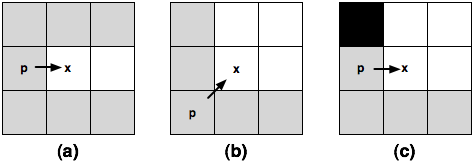
\includegraphics[width=0.95\columnwidth]
			{diagrams/pruning.png}
       \end{center}
	\vspace{-3pt}
       \caption{(a) When the move from $p$ to $x$ is straight only one natural neighbour remains.
(b) When the move from $p$ to $x$ is diagonal, three natural neighbours remain. (c) Obstacles around $x$
cause some neighbours to become forced. }
       \label{fig:pruning}
\end{figure}

We illustrate these rules in Figure~\ref{fig:pruning}(a) and ~\ref{fig:pruning}(b).
Observe that to test each rule we need to look only at
the neighbours of the current node $x$. 
Pruned neighbours are marked in grey. Remaining neighbours, marked
white, are called the \emph{natural} successors of node $x$.  
In Figure~\ref{fig:pruning}(c) we show
that obstacles can modify the list of successors for $x$:
when the alternative path $\pi' = \langle p, y, n \rangle$ is
not valid, but $\pi = \langle p, x, n \rangle$ is, we will refer to $n$ as
a \emph{forced} successor of $x$.
The set of forced successors in Figure~\ref{fig:pruning}(c) is different
to the set identified in~\cite{harabor11b}. 
In that work we assumed corner-cutting (a.k.a taking a diagonal shortcut around a corner) is allowed.
Here we explicitly require that both $\pi$ and $\pi'$ respect 
any such domain-specific movement rules.
When corner-cutting is not allowed this change has the following effect:
only straight steps from $p$ to $x$ may produce forced neighbours and each $x$ may have 
up to 4 such neighbours.
This change preserves optimality; the argument is identical to 
the one in~\cite{harabor11b}.

\textbf{Jumping Rules:}
JPS applies to each forced and natural neighbour of the current node $x$ a simple
``jumping'' procedure; the objective is to replace each neighbour $n$ with an 
alternative successor $n'$ that is further away. Precise details are given
in~\cite{harabor11b}; we summarise the idea here using a short example:

\begin{example}
In Figure~\ref{fig:pruning}(a) pruning reduces the number
of successors of $x$ to a single node $n$.
JPS exploits this property to immediately and recursively
explore $n$.
If the recursion stops due to an obstacle that blocks further progress
(which is frequently the case), all nodes on the failed path, including $n$, are ignored
and nothing is generated.
Otherwise the recursion leads to a node $n'$ which has a forced
neighbour (or which is the goal). JPS generates $n'$ as a successor of $x$; 
effectively allowing the search to ``jump'' from $x$ directly to $n'$ -- without adding
to the open list any intermediate nodes from along the way.
In Figure~\ref{fig:pruning}(b) node $x$ has three natural neighbours: two straight and one diagonal.
We recurse over the diagonal neighbour only if both straight neighbours produce
failed paths. This ensures we do not miss any potential turning points of the optimal path.
\end{example}

\begin{figure}[tb]
       \begin{center}
		   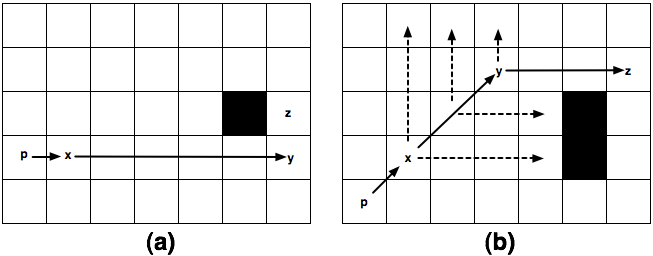
\includegraphics[width=0.95\columnwidth]
			{diagrams/jumping.png}
       \end{center}
	\vspace{-3pt}
       \caption{(a) A straight jump from $x$ to $y$; the recursion stops due to node $z$ which is forced.
(b) A diagonal jump from $x$ to $y$; the recursion stops due to a non-failed straight jump. Continuing 
would mean missing a potential turn due to $z$.}
       \label{fig:jumping}
\end{figure}

In Figure~\ref{fig:jumping}(a) we illustrate a straight jump and in \ref{fig:jumping}(b) a diagonal jump. 
By jumping, JPS is able to move quickly over the map 
without inserting nodes in the A* open list.
This is doubly beneficial as (i) it reduces the number of operations 
and (ii) it reduces the number of nodes in the queue, 
making each queue operation cheaper.  
Notice that this version of JPS is performed entirely online, involves no preprocessing and has no memory overhead.  


\begin{tikzpicture}
  \creategrid{9}{7}
%  \drawobstacle{2}{8}
%  \draw[->] (0.7,2.7) -- (1.3,3.3);
  \drawgridnode{3}{5}{$x$}
  \drawobstacle{8}{5}
  \drawobstacle{8}{4}
  \drawobstacle{8}{3}
  \drawgridnode{1}{7}{$1$}
  \draw[->] (2.3,4.7) -- (0.7,6.3);
  \drawgridnode{3}{7}{$2$}
  \draw[->] (2.5,4.7) -- (2.5,6.3);
  \drawgridnode{4}{6}{$3$}
  \draw[->] (2.7,4.7) -- (3.3,5.3);
  \drawgridnode{6}{5}{$4$}
  \draw[->] (2.7,4.5) -- (5.3,4.5);
  \drawgridnode{6}{2}{$5$}
  \draw[->] (2.7,4.3) -- (5.3,1.7);
  \drawgridnode{3}{1}{$6$}
  \draw[->] (2.5,4.3) -- (2.5,0.7);
  \drawgridnode{1}{3}{$7$}
  \draw[->] (2.3,4.3) -- (0.7,2.7);
  \drawgridnode{1}{5}{$8$}
  \draw[->] (2.3,4.5) -- (0.7,4.5);
\end{tikzpicture} \qquad
\begin{tikzpicture}
  \creategrid{9}{7}
%  \drawobstacle{2}{8}
%  \draw[->] (0.7,2.7) -- (1.3,3.3);
  \drawgridnode{3}{5}{$x$}
  \drawobstacle{8}{5}
  \drawobstacle{8}{4}
  \drawobstacle{8}{3}
% \drawgridnode{1}{7}{$1$}
% \draw[->] (2.3,4.7) -- (0.7,6.3);
% \drawgridnode{3}{7}{$2$}
% \draw[->] (2.5,4.7) -- (2.5,6.3);
% \drawgridnode{4}{6}{$3$}
% \draw[->] (2.7,4.7) -- (3.3,5.3);
% \drawgridnode{6}{5}{$4$}
% \draw[->] (2.7,4.5) -- (5.3,4.5);
  \drawgridnode{6}{2}{$y$}
  \draw[->] (2.7,4.3) -- (5.3,1.7);
% \drawgridnode{3}{1}{$6$}
% \draw[->] (2.5,4.3) -- (2.5,0.7);
% \drawgridnode{1}{3}{$7$}
% \draw[->] (2.3,4.3) -- (0.7,2.7);
% \drawgridnode{1}{5}{$8$}
% \draw[->] (2.3,4.5) -- (0.7,4.5);
  \draw[green,line width=2pt] (0,3.5) -- (9,3.5);
  \draw[green,line width=2pt] (4.5,0) -- (4.5,7);
  \drawgridnode{5}{4}{$t$}
  \drawgridnode{4}{4}{$y'$}
\end{tikzpicture}%
% EOF

\chapter{Conclusion}
\label{cha:conc}
Summary your thesis and discuss what you are going to do in the future in Section~\ref{sec:future}.


\section{Future Work}
\label{sec:future}
Good luck.




\section{Acknowledgements}
\label{sec::ack}
We thank Patrik Haslum for taking the time to read and comment on 
an early revision of this paper.
NICTA is funded by the Australian Government through the Department of
Communications and the Australian Research Council through the ICT Centre of
Excellence Program.


\bibliographystyle{aaai/aaai}
\bibliography{references}

\end{document}
